\renewcommand{\baselinestretch}{2} \small\normalsize
\chapter{Environmental Impacts}\label{chapter_env}
Before developing a statistical model, we need to understand which environmental factors affect propagation. Multipath, clutter, and sea spikes are all induced by reflections from the sea surface while changes in the index of refraction cause electromagnetic waves to bend. We will first describe the various earth models that are used along with the propagation geometry that follows from these models. Next we will discuss refractivity and anomalous propagation before covering the reflective effects of multipath, clutter, and sea spikes. We will close this chapter with a discussion of ship target RCS fluctuations.

\section{Earth Models}
The earth can be modeled as flat to simplify calculations, as a sphere to capture horizon effects for long range propagation, or as an ellipsoid to provide additional geometric accuracy. In general, the standard model is spherical with the 4/3 earth radius approximation.

\subsection{Flat Earth}
The flat earth model is valid only for short ranges as there is no concept of the RADAR horizon. The geometry provides a simple planar surface such that the local tangent plane is equivalent at both the transmitter and target. This model is shown in Figure \ref{env_fig:1}, where $h_1$ is the altitude of the transmitter, $h_2$ is the altitude of the target, $R$ is the slant range, $\alpha$ is the depression angle, and $\chi$ is the grazing angle. Also shown in this figure is a single multipath bounce off the surface (the direct path between the transmitter and receiver is not shown). 

\begin{figure}[H]
  \begin{center}
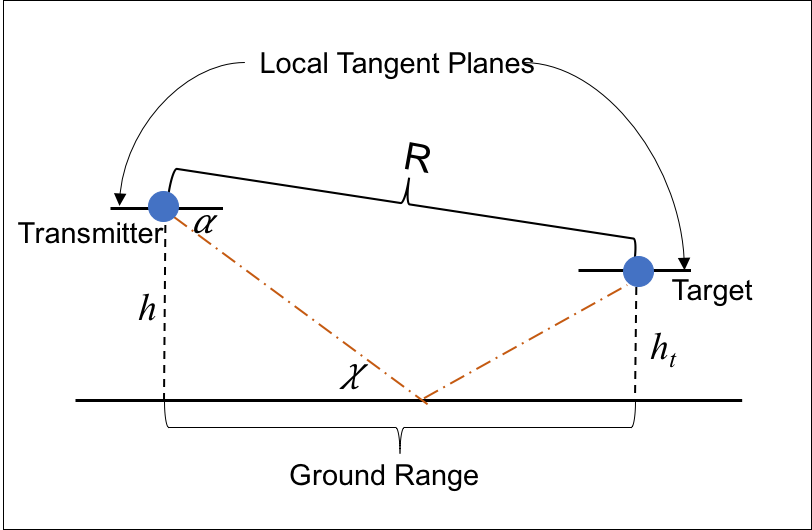
\includegraphics[width=4in]{../media/multistatic/flat_earth_geometry.png}
  \end{center}
  \renewcommand{\baselinestretch}{1} \small\normalsize
  \begin{quote}
    \caption[Flat Earth Geometry]{Flat Earth Geometry\label{env_fig:1}}
  \end{quote}
\end{figure}
\renewcommand{\baselinestretch}{2} \small\normalsize
Flat earth approximations are typically used for initial back of the envelope calculations but should not be used to assess critical performance characteristics. 

\subsection{Spherical Earth}
The spherical earth model assumes the earth is a sphere, with a constant radius $r_e = 6370$ km and is shown in Figure \ref{env_fig:2}. In this figure, $r_e'$ represents the effective radius of the earth.

\begin{figure}[H]
  \begin{center}
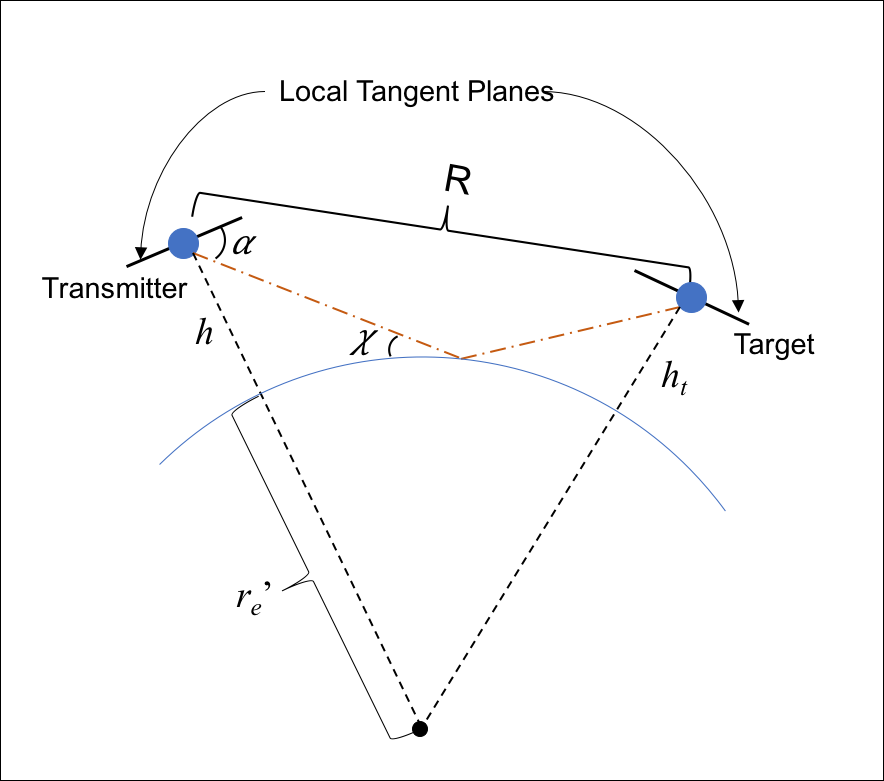
\includegraphics[width=4in]{../media/multistatic/spherical_earth_geometry.png}
  \end{center}
  \renewcommand{\baselinestretch}{1} \small\normalsize
  \begin{quote}
    \caption[Spherical Earth Geometry]{Spherical Earth Geometry\label{env_fig:2}}
  \end{quote}
\end{figure}
\renewcommand{\baselinestretch}{2} \small\normalsize
The curvature of the earth changes the reference planes between the transmitter and target, so that the local tangent planes are not equivalent.

\subsection{WGS-84 Earth}
The World Geodetic System (WGS) is an earth fixed standard coordinate system developed in 1984 and the current standard is identified as WGS-84 \cite{dod_wgs84}. This model is not generally used for RADAR calculations as it complicates analysis beyond the spherical earth model and the difference between the two models is negligible compared to the uncertainty in the refractive index profile. In cases where we desire the additional geometry accuracy, such as RADAR horizon calculations at a particular location on the earth, we can follow the spherical earth model but use the local radius of curvature from the WGS-84 earth model as $r_e$.

\subsection{4/3 Earth Model}
Due to the refractive index of the atmosphere, the propagation path of an electromagnetic wave will curve. Under the assumption of standard atmospheric conditions, the propagation path can be approximated as a straight line if an effective radius of the earth is used, $r_e' = 4/3 r_e$ \cite{blake_radar}, \cite{nathanson_radar}. This is referred to as the 4/3 earth model and is used in most analytical calculations.

As stated above, we can increase geometric accuracy for locality by using the local radius of curvature from the WGS-84 model for $r_e$.

\section{Geometry}
The earth model used defines the propagation geometry. The geometric aspects of most importance are the grazing angle, depression angle, and RADAR horizon. The grazing and depression angles are important in computing the reflection coefficients and beam intersection area for both clutter and multipath and the RADAR horizon bounds the propagation range.

\subsection{Grazing and Depression Angles}
The grazing and depression angles are both defined for rays intersecting the earth as shown in Figure \ref{env_fig:2}. The depression angle, $\alpha$ is the angle from the local horizontal plane at the transmitter and is given by Equation \ref{env_eq:1} \cite{nathanson_radar}.
\begin{equation}
  \label{env_eq:1}
  \alpha = \sin^{-1}\left(\frac{2r_e'h_1 + h_1^2 + R^2}{2R\left[r_e' + h_1 \right]} \right)
  \end{equation}
  
The grazing angle, $\chi$, is the angle from the local horizontal plane at the target and is given by Equation \ref{env_eq:2} \cite{nathanson_radar}.
  \begin{equation}
  \label{env_eq:2}
  \chi = \sin^{-1}\left(\frac{h_1}{R}\left[1 + \frac{h_1}{2r_e'} \right] - \frac{R}{2r_e'} \right)
  \end{equation}
  
In the flat earth case, the grazing and depression angles are equal. The curvature of the earth changes the local tangent plane reference, so they are not equal in the case of a spherical or ellipsoidal earth.
  
\subsection{RADAR Horizon}
The curvature of the earth puts an upper limit on the distance an electromagnetic wave can travel before intercepting the earth. The range to the horizon, $R_h$, is given by Equation \ref{env_eq:3}. Slant ranges greater than this distance will be clipped by the earth and not reach the target unless anomalous propagation conditions (ducting) are present.
  \begin{equation}
  \label{env_eq:3}
  R_h = \sqrt{2r_e'h_1 + h_1^2} + \sqrt{2r_e'h_2 + h_2^2}
  \end{equation}
In this equation, $h_1$ is the altitude of the transmitter and $h_2$ is the altitude of the target.

Because an electromagnetic wave consists of a finite bundle of rays rather than a single ray, the physical clipping by the horizon is gradual rather than instantaneous. The impact of the horizon should be modeled by a smooth rolloff rather than a step function.
  
\section{Anomalous Refraction Effects}
As stated previously, electromagnetic wave propagate along a curved path which we can approximate as linear under standard atmosphere and the 4/3 earth model. The refractive index gradient is negative in this case (the index of refraction decreases with increasing altitude); when the gradient changes, the linear approximation is no longer valid and we have anomalous propagation. 

There are 3 classes of anomalous propagation, subrefraction (when the gradient of the index of refraction becomes positive so that rays bend upwards), superrefraction (when the gradient of the index of refraction becomes more negative so that rays bend more strongly downwards), and ducting (the gradient of the index of refraction becomes negative enough to hit a critical point where the radius of curvature of the ray becomes less than the radius of curvature of the earth and the ray becomes trapped as in a waveguide) \cite{blake_radar}.

Because an atmospheric duct acts like a waveguide, electromagnetic waves can propagate significantly beyond the horizon in the presence of a duct. Figure \ref{env_fig:2z} shows how the difference in how the propagation factor is impacted by standard atmosphere and a 20 m duct.
\begin{figure}[H]
  \begin{center}
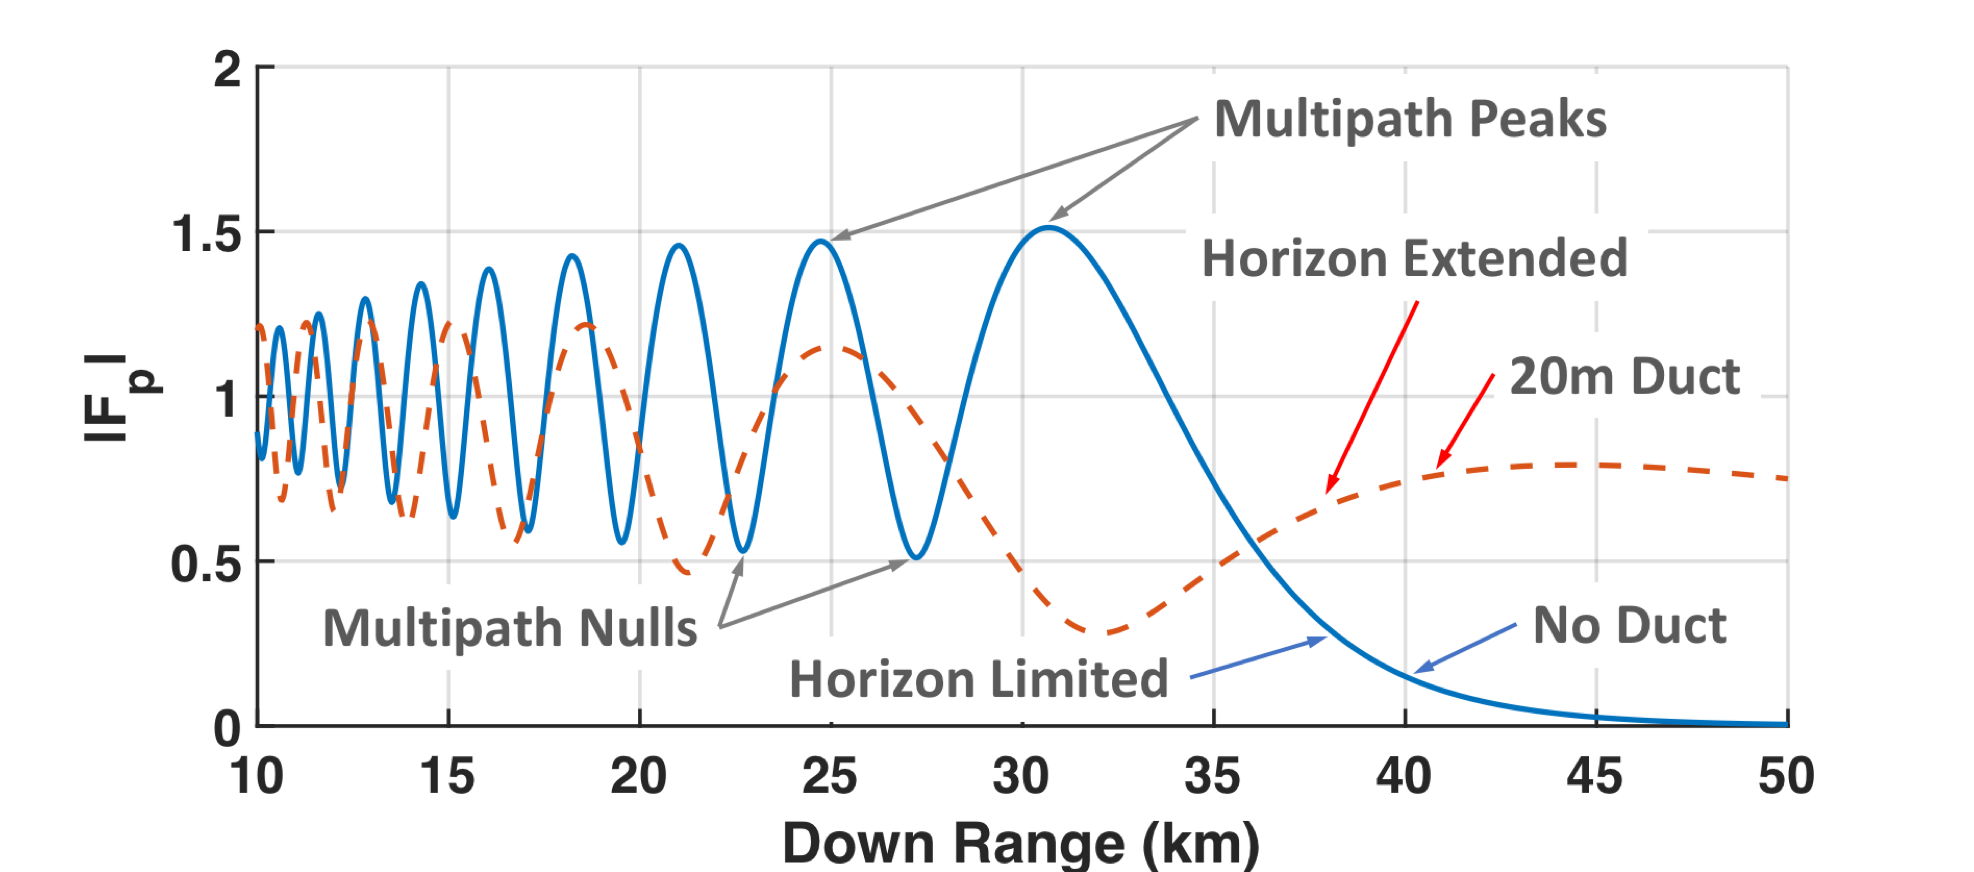
\includegraphics[width=5in]{../media/multistatic/multipath.png}
  \end{center}
  \renewcommand{\baselinestretch}{1} \small\normalsize
  \begin{quote}
    \caption[Propagation Factors for Standard Atmosphere vs. 20 m Duct]{Propagation Factors for Standard Atmosphere vs. 20 m Duct\label{env_fig:2z}}
  \end{quote}
\end{figure}
\renewcommand{\baselinestretch}{2} \small\normalsize

\section{Multipath}
Multipath refers to reflections from the surface of the earth resulting in many paths between the transmitter and the target. When these paths are in phase, the signal at the target is amplified. When these paths are out of phase, the signal is reduced and referred to as a multipath null.

\subsection{2-Ray Model}
The 2-Ray Model for multipath is shown in Figure \ref{env_fig:3}, using a flat earth geometry to simplify the explanation. In this model, the two rays are the direct path from the transmitter to the target and a single multipath bounce from the surface between the transmitter and target.
\begin{figure}[H]
  \begin{center}
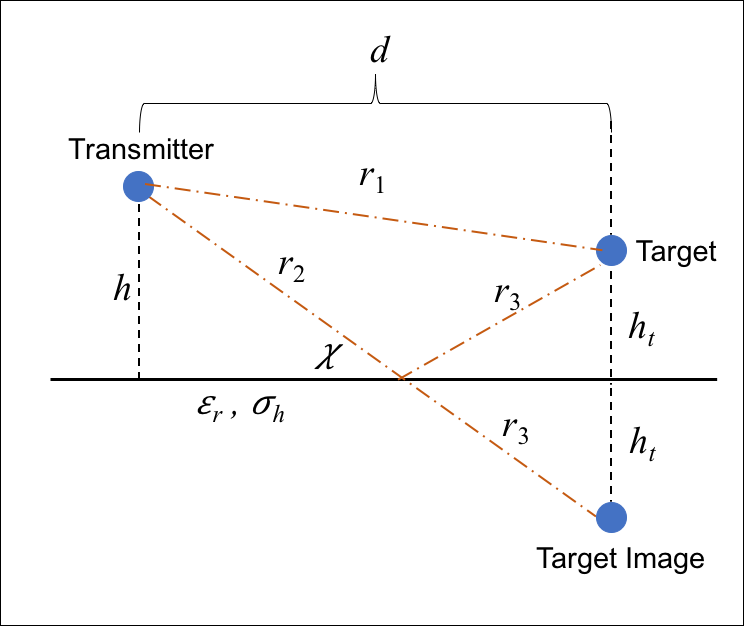
\includegraphics[width=4in]{../media/multistatic/two_ray_multipath_model.png}
  \end{center}
  \renewcommand{\baselinestretch}{1} \small\normalsize
  \begin{quote}
    \caption[Two Ray Multipath Model]{Two Ray Multipath Model\label{env_fig:3}}
  \end{quote}
\end{figure}
\renewcommand{\baselinestretch}{2} \small\normalsize
The sea surface is characterized by its dielectric constant, $\epsilon_r$, and the height variance, $\sigma_h$, which will result in a reflection coefficient, $\Gamma_t$. We can characterize the multipath ray by using the image of the target.

Using plane waves and following \cite{lohrmann_rcs}, we can use superposition and express the combination of the rays as a propagation factor, $F_p$:
  \begin{equation}
  \label{env_eq:3b}
F_p = e^{jkr_1} + \Gamma_te^{jk\left(r_2 + r_3\right)}
\end{equation}

This is a simplified approach that captures the "effect" of going through multipath peaks and nulls, but does not include cylindrical spreading of the wavefront as it propagates.

In this expression, the result is dependent on the phase difference between the path distances $r_1$ and $r_2 + r_3$. This means we will have a multipath null (destructive interference) whenever $k\left(r_1 - r_2 - r_3\right) = (2m + 1)\pi$ and we will have a multipath peak (constructive interference) whenever $k\left(r_1 - r_2 - r_3\right) = 2m\pi$. From geometry, we can see that $r_1 = \sqrt{d^2 + (h_1-h_2)^2}$ and $r_2 + r_3 = \sqrt{d^2 + (h_1+h_2)^2}$

This model for multipath is generated from a flat earth geometry. We can provide a spherical earth correction by modifying the target altitude \cite{blake_radar} such that
\begin{equation}
  \label{env_eq:3r}
h_2' = h_2 + \frac{d}{2r_e'}
\end{equation}

Figure \ref{env_fig:3t} shows an example of the propagation factor from the two ray multipath model with the spherical earth correction applied. Here $h_1 = 15m$, $h_2 = 15m$, $f = 35$ GHz, and $\Gamma_t = 1$. 
\begin{figure}[H]
  \begin{center}
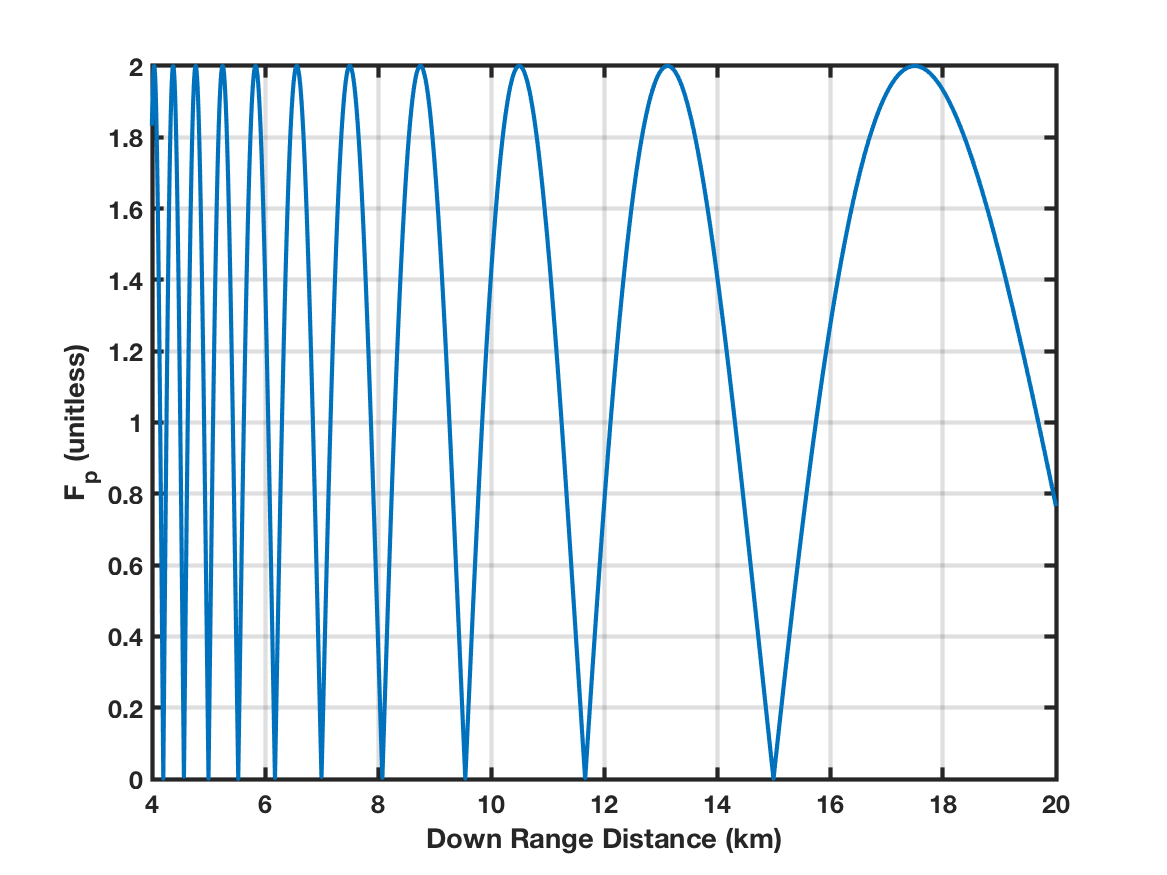
\includegraphics[width=4in]{../media/multistatic/two_ray_multipath_results.png}
  \end{center}
  \renewcommand{\baselinestretch}{1} \small\normalsize
  \begin{quote}
    \caption[Two Ray Multipath Model Results]{Two Ray Multipath Model Results\label{env_fig:3t}}
  \end{quote}
\end{figure}
\renewcommand{\baselinestretch}{2} \small\normalsize

\subsection{Reflection Coefficient}
From \cite{miller_reflection}, we can express the rough sea surface reflection coefficient, $\rho$, by Equation \ref{env_eq:4}. 
  \begin{equation}
  \label{env_eq:4}
\rho = \left|\frac{\bar{E}}{E_\delta \Gamma} \right| = e^{-2\left[2\pi g \right]^2}I_0\left( 2\left[2\pi g \right]^2\right) 
\end{equation}
This is commonly referred to as the "Miller-Brown approximation". In this equation, $g = \sigma_h\sin(\chi)/\lambda$, $\bar{E}$ is the average electric field reflected from the surface, $E_\delta$ is the incident electric field, $\Gamma$ is the smooth (Fresnel) reflection coefficient, and $I_0$ is the modified Bessel function of the first kind.

The smooth reflection coefficient depends on the polarization of the incident wave and is given by Equation \ref{env_eq:5} for horizontal polarization and by Equation \ref{env_eq:6} for vertical polarization.
  \begin{equation}
  \label{env_eq:5}
 \Gamma_h = \frac{\sin(\chi)- \sqrt{\epsilon_r - \cos^2(\chi)}}{\sin(\chi) + \sqrt{\epsilon_r - \cos^2(\chi)}}
  \end{equation}
  
  \begin{equation}
  \label{env_eq:6}
 \Gamma_v = \frac{\sin(\chi)- \sqrt{\frac{\epsilon_r - \cos^2(\chi)}{\epsilon_r^2}}}{\sin(\chi) + \sqrt{\frac{\epsilon_r - \cos^2(\chi)}{\epsilon_r^2}}}
  \end{equation}
In these equations, $\epsilon_r$ is the relative permittivity of the ocean and is given by Equation \ref{env_eq:7} at $20^{\circ}$ C and $3.6\%$ salinity for an electromagnetic wave with temporal frequency $f$. 
  
\begin{equation}
  \label{env_eq:7}
\epsilon_r = \left[\frac{64.18}{1 + 3.30523\times 10^{-21}f^2} + 4.9 \right] + j\left[\frac{3.689792\times 10^{-9}f}{1 + 3.30523\times 10^{-21}f^2} + \frac{9.4\times 10^{10}}{f} \right]
  \end{equation}
  
The total reflection coefficient, $\Gamma_t$ is then the product of the rough and smooth reflection coefficients, $\Gamma_t = \rho\Gamma_h$ or $\Gamma_t = \rho\Gamma_v$.

\section{Clutter}
Clutter is the backscattered signal from the sea surface and the unwanted signal strength can be found from the RADAR range equation using the product of the backscatter cross section, $\sigma^0$ and the clutter cell area, $A_c$. The area will depend on if the signal is beam limited or pulse limited. The Signal to Clutter Ratio (SCR) is the ratio of the power received from the signal to the power received from clutter and is a good indicator of overall performance.

\subsection{NRL Model for $\sigma^0$}
There are many models for estimating the backscatter cross section at various sea states \cite{blake_radar} \cite{richards_radar} \cite{nathanson_radar}. In 2012, an empirical model was developed by NRL that minimized differences with the extensive experimental database \cite{gregers-hansen_clutter} and that model will be presented here. Equation \ref{env_eq:7a} provides the model for $\sigma^0$ and Table \ref{env_tab:0} lists the various constants used in the equation with $f$ the radar frequency in GHz, $SS$ the sea state, and $\alpha$ the grazing angle in degrees.

\begin{equation}
\begin{gathered}
  \sigma^0 = c_1 + c_2 \log_{10}(\sin(\alpha))+\frac{\left(27.5 + c_3\alpha\right)\log_{10}(f)}{1+0.95\alpha}+\\
  c_4\left(1 + SS \right)^{1/\left(2+0.085\alpha + 0.033SS\right)}
 + c_5\alpha^2 
 \end{gathered}
 \label{env_eq:7a}
  \end{equation}
  
  \begin{table}[H]
  \begin{center}
      \renewcommand{\baselinestretch}{1} \small\normalsize
  \begin{quote}
    \caption[Constants in NRL Clutter Model]{Constants in NRL Clutter Model\label{env_tab:0}}
  \end{quote}
  \begin{tabular} {|c | c | c|}
    \hline
  \bf{Constant} & \bf{Horizontal Polarization}n & \bf{Vertical Polarization} \\ \hline
  $c_1$ & -73.0 & -50.79  \\ \hline
  $c_2$ & 20.78 & 25.93  \\ \hline
  $c_3$ & 7.351 & 0.7093 \\ \hline
  $c_4$ & 25.65 & 21.58  \\ \hline
  $c_5$ & 0.00540 & 0.00211 \\ \hline
\end{tabular}
\end{center}
\end{table}
\renewcommand{\baselinestretch}{2} \small\normalsize
  
\subsection{Beam Limited Case}
In the beam limited case, the pulse width is large compared to the projection of the beamwidth on the surface and $A_c$ is then only limited by the geometric illuminated area of the beam.

Figure \ref{env_fig:3z} shows an example of the SCR with the beamlimited case. Here the crossover points are also identified where the signal is 12dB, 6dB, 3dB, and 0dB larger than the clutter.
\begin{figure}[H]
  \begin{center}
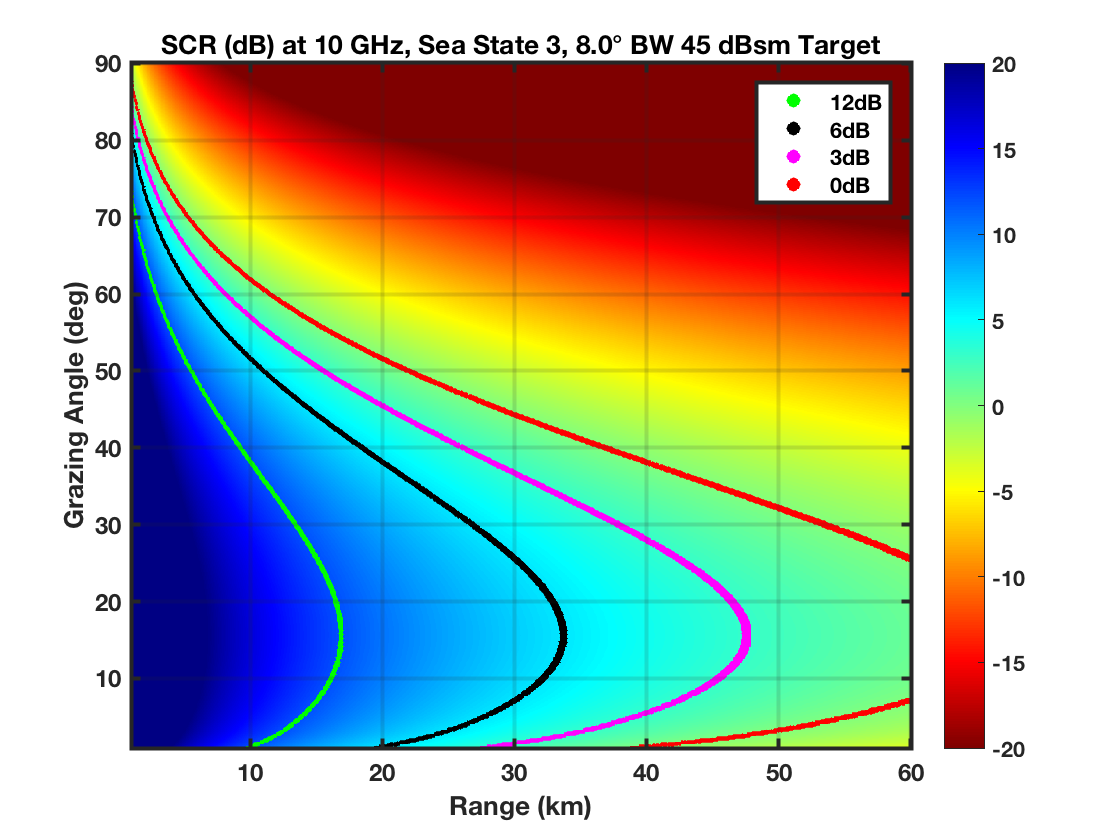
\includegraphics[width=4in]{../media/multistatic/scr.png}
  \end{center}
  \renewcommand{\baselinestretch}{1} \small\normalsize
  \begin{quote}
    \caption[SCR Example for the Beam Limited Case]{SCR Example for the Beam Limited Case\label{env_fig:3z}}
  \end{quote}
\end{figure}
\renewcommand{\baselinestretch}{2} \small\normalsize

\subsection{Pulse Limited Case}
In the pulse limited case, the pulse width is short compared to the projection of the beamwidth on the surface and $A_c$ is then limited by the projected pulse width.

\section{Target RCS}
\subsection{Point Targets}
\subsection{Complex Targets}
\subsection{Fluctuating Target Models}
Fluctuating target RCS models were developed to describe the fluctuations observed in RCS due to motion of the ship in the waves. These models should only be applied to single point targets, as multi-scatterer targets will inherently include the dependence on motion and aspect angle.

\subsubsection{Target RCS PDF}
For traditional monostatic RADAR systems, work done by Jess Marcum and Peter Swerling provided statistical models for the RCS of targets in the ocean\cite{richards_radar}. There are $4$ Swerling cases that are generally considered, using $2$ different decorrelation time lengths and $2$ different PDFs as shown in Table \ref{env_tab:1}. 

\begin{table}[H]
  \begin{center}
      \renewcommand{\baselinestretch}{1} \small\normalsize
  \begin{quote}
    \caption[Swerling Fluctuating Target RCS Model Description]{Swerling Fluctuating Target RCS Model Description\label{env_tab:1}}
  \end{quote}
  \begin{tabular} {|c | c | c |}
    \hline
  \bf{Case} & \bf{Decorrelation Time Length} & \bf{Chi-squared PDF Degree} \\ \hline
  1 &Long (Scan to Scan) &2 \\ \hline
  2 &Short (Pulse to Pulse) &2 \\ \hline
  3 &Long (Scan to Scan) &4 \\ \hline
  4 &Short (Pulse to Pulse) &4 \\ \hline
\end{tabular}
\end{center}
\end{table}
\renewcommand{\baselinestretch}{2} \small\normalsize
The Chi-squared of degree $2$ or exponential PDF applies to the case with many randomly distributed small scatterers with none dominant and the Chi-squared of degree $4$ PDF applies to the case with a single dominant scatterer and many small scatterers. These PDFs are shown in Figure \ref{env_fig:4}.
\begin{figure}[H]
  \begin{center}
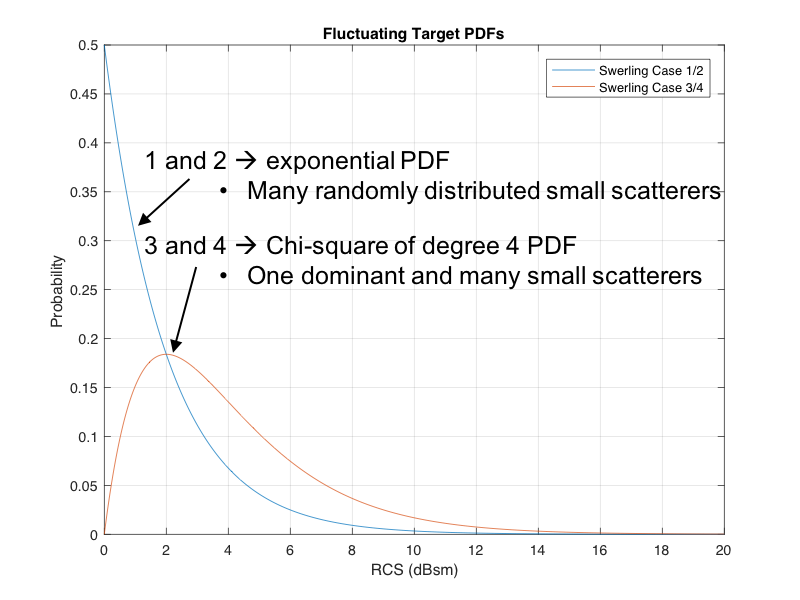
\includegraphics[width=4in]{../media/multistatic/swerling_pdfs.png}
  \end{center}
  \renewcommand{\baselinestretch}{1} \small\normalsize
  \begin{quote}
    \caption[Swerling Target Fluctuation Model PDFs]{Swerling Target Fluctuation Model PDFs\label{env_fig:4}}
  \end{quote}
\end{figure}
\renewcommand{\baselinestretch}{2} \small\normalsize

The long decorrelation time applies when the target RCS can be considered constant over the time the RADAR performs a single scan and the short decorrelation time applies when the target RCS changes on a pulse to pulse basis. Many modern RADAR systems operate in frequency agile modes where the carrier frequency is changed each pulse, in which case the decorrelation time can be considered to be short. A fluctuating signal can have a significant effect on the probability of detection, $P_d$, as seen in Figure \ref{env_fig:5}. This figure shows $P_d$ as a function of SNR for the nonfluctating case and each of the $4$ Swerling cases and demonstrates that using the wrong PDF can result in significantly overestimating $P_d$.
\begin{figure}[H]
  \begin{center}
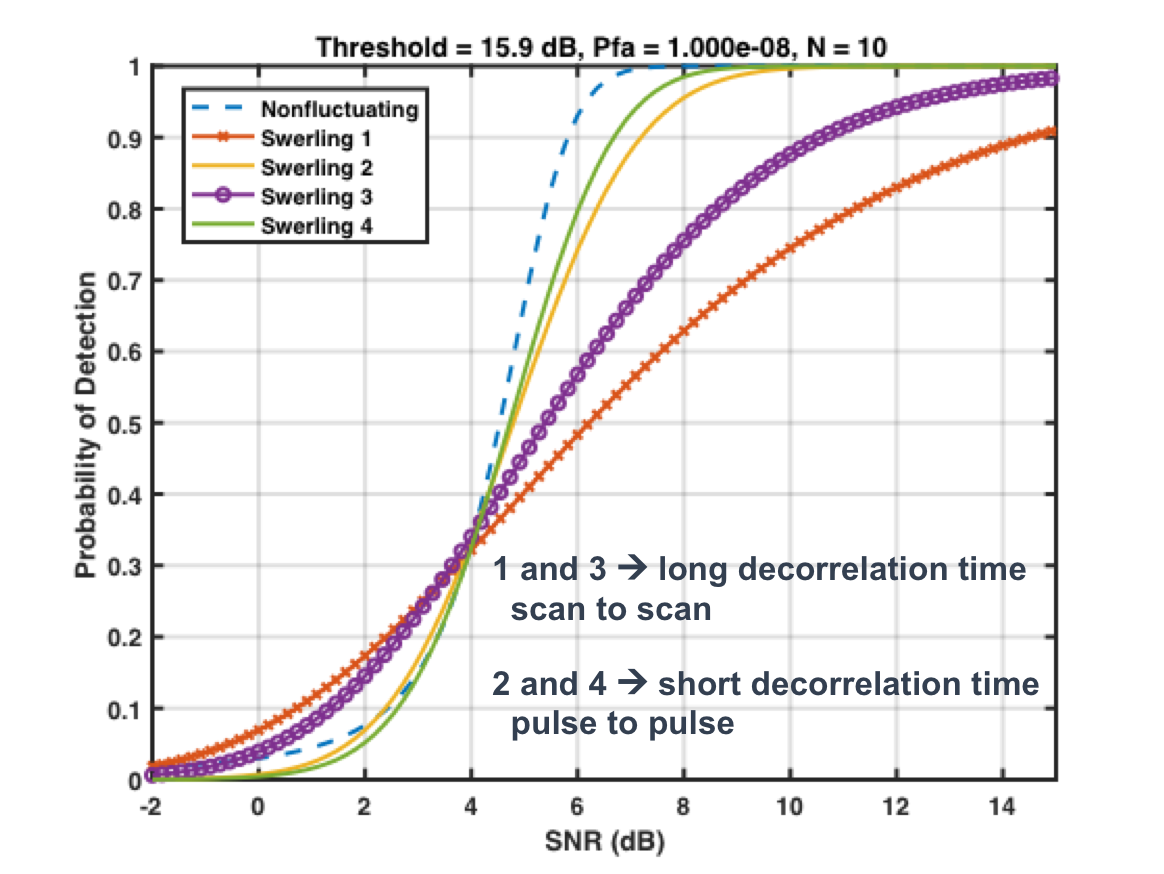
\includegraphics[width=4in]{../media/multistatic/swerling_pd.png}
  \end{center}
  \renewcommand{\baselinestretch}{1} \small\normalsize
  \begin{quote}
    \caption[Swerling Target Fluctuation Model Probability of Detection]{Swerling Target Fluctuation Model Probability of Detection\label{env_fig:5}}
  \end{quote}
\end{figure}
\renewcommand{\baselinestretch}{2} \small\normalsize

Figure \ref{env_fig:4} also shows that $P_d$ is higher with a dominant scatterer than with a collection of uniform scatterers and that it is higher for a short decorrelation time than a long decorrelation time. We can force the decorrelation time to be short by operating in a frequency agile mode, but we generally have no control over the target configuration.

\subsubsection{Generating RCS Fluctuations}
Modeling the RCS for a Swerling fluctuating target is straightforward. We can generate random variables following a Chi-squared distribution of degree $n$ by the sum of $n$ squared normally distributed random variables with zero mean and unit variance. The mean of the Chi-squared distribution is equal to the degree, so to force the mean to a specified deterministic RCS mean, we need to add the deterministic mean and subtract the degree.

Swerling cases 1 and 2 follow a Chi-squared distribution of degree 2. To generate a random variable, $w_{12}$, for our RCS, we need to generate 2 normally distributed random variables, $u_1$ and $u_2$. Then, $w_{12}$ is given by Equation \ref{env_eq:8}, where $\sigma$ is the deterministic RCS value.
\begin{equation}
  \label{env_eq:8}
w_{12} = u_1^2 + u_2^2 + \sigma - 2
  \end{equation}

Swerling cases 3 and 4 follow a Chi-squared distribution of degree 4. To generate a random variable, $w_{34}$, for our RCS, we need to generate 4 normally distributed random variables, $u_1$, $u_2$, $u_3$, and $u_4$. Then, $w_{34}$ is given by Equation \ref{env_eq:9}, where $\sigma$ is again the deterministic RCS value.
\begin{equation}
  \label{env_eq:9}
w_{34} = u_1^2 + u_2^2 + u_3^2 + u_4^2 + \sigma - 4
  \end{equation}
  
The decorrelation time then determines when to perform the random draws; this can be every pulse, every CPI, or at some predetermined time interval. When we have multiple transmitters, we need to be careful about when to schedule the random RCS draws so that one actor does not influence the others.  